\documentclass[conference,compsoc]{IEEEtran}
\usepackage{cite}
\usepackage[english]{babel}
\usepackage[pdftex]{graphicx}
\DeclareGraphicsExtensions{.pdf,.jpeg,.png}
\usepackage{amsmath}
\usepackage[caption=false,font=footnotesize,labelfont=sf,textfont=sf]{subfig}
\usepackage{url}
\hyphenation{op-tical net-works semi-conduc-tor}

\makeatletter
\def\endthebibliography{%
	\def\@noitemerr{\@latex@warning{Empty `thebibliography' environment}}%
	\endlist
}
\makeatother

\begin{document}
\title{Data Driven Project Management \\ Predicting the Development Time}


\author{\IEEEauthorblockN{Marko Prelevikj}
	\IEEEauthorblockA{Faculty of Computer and Information Science\\
		University of Ljubljana\\
		Ljubljana, Slovenia\\
		Email: mp2638@stuent.uni-lj.si}
}

\maketitle

\begin{abstract}
The abstract goes here.
\end{abstract}

\IEEEpeerreviewmaketitle

\section{Introduction}
explain PMO's problems
\section{Model data}
JIRA data briefly and what the model is consisted of

\section{Testing model quality}
Present different the results (MAE, RMSE, R2) obtained by different regressors.

\section{Model Explainability}
Write about feature importance and how to explain the made decisions.


\section{Conclusion}
Quick recap of the problem and how we solved it.
XGBoost~\cite{chen2016xgboost}, SHAP~\cite{lundberg2020local2global}.

\begin{figure}[!t]
\centering
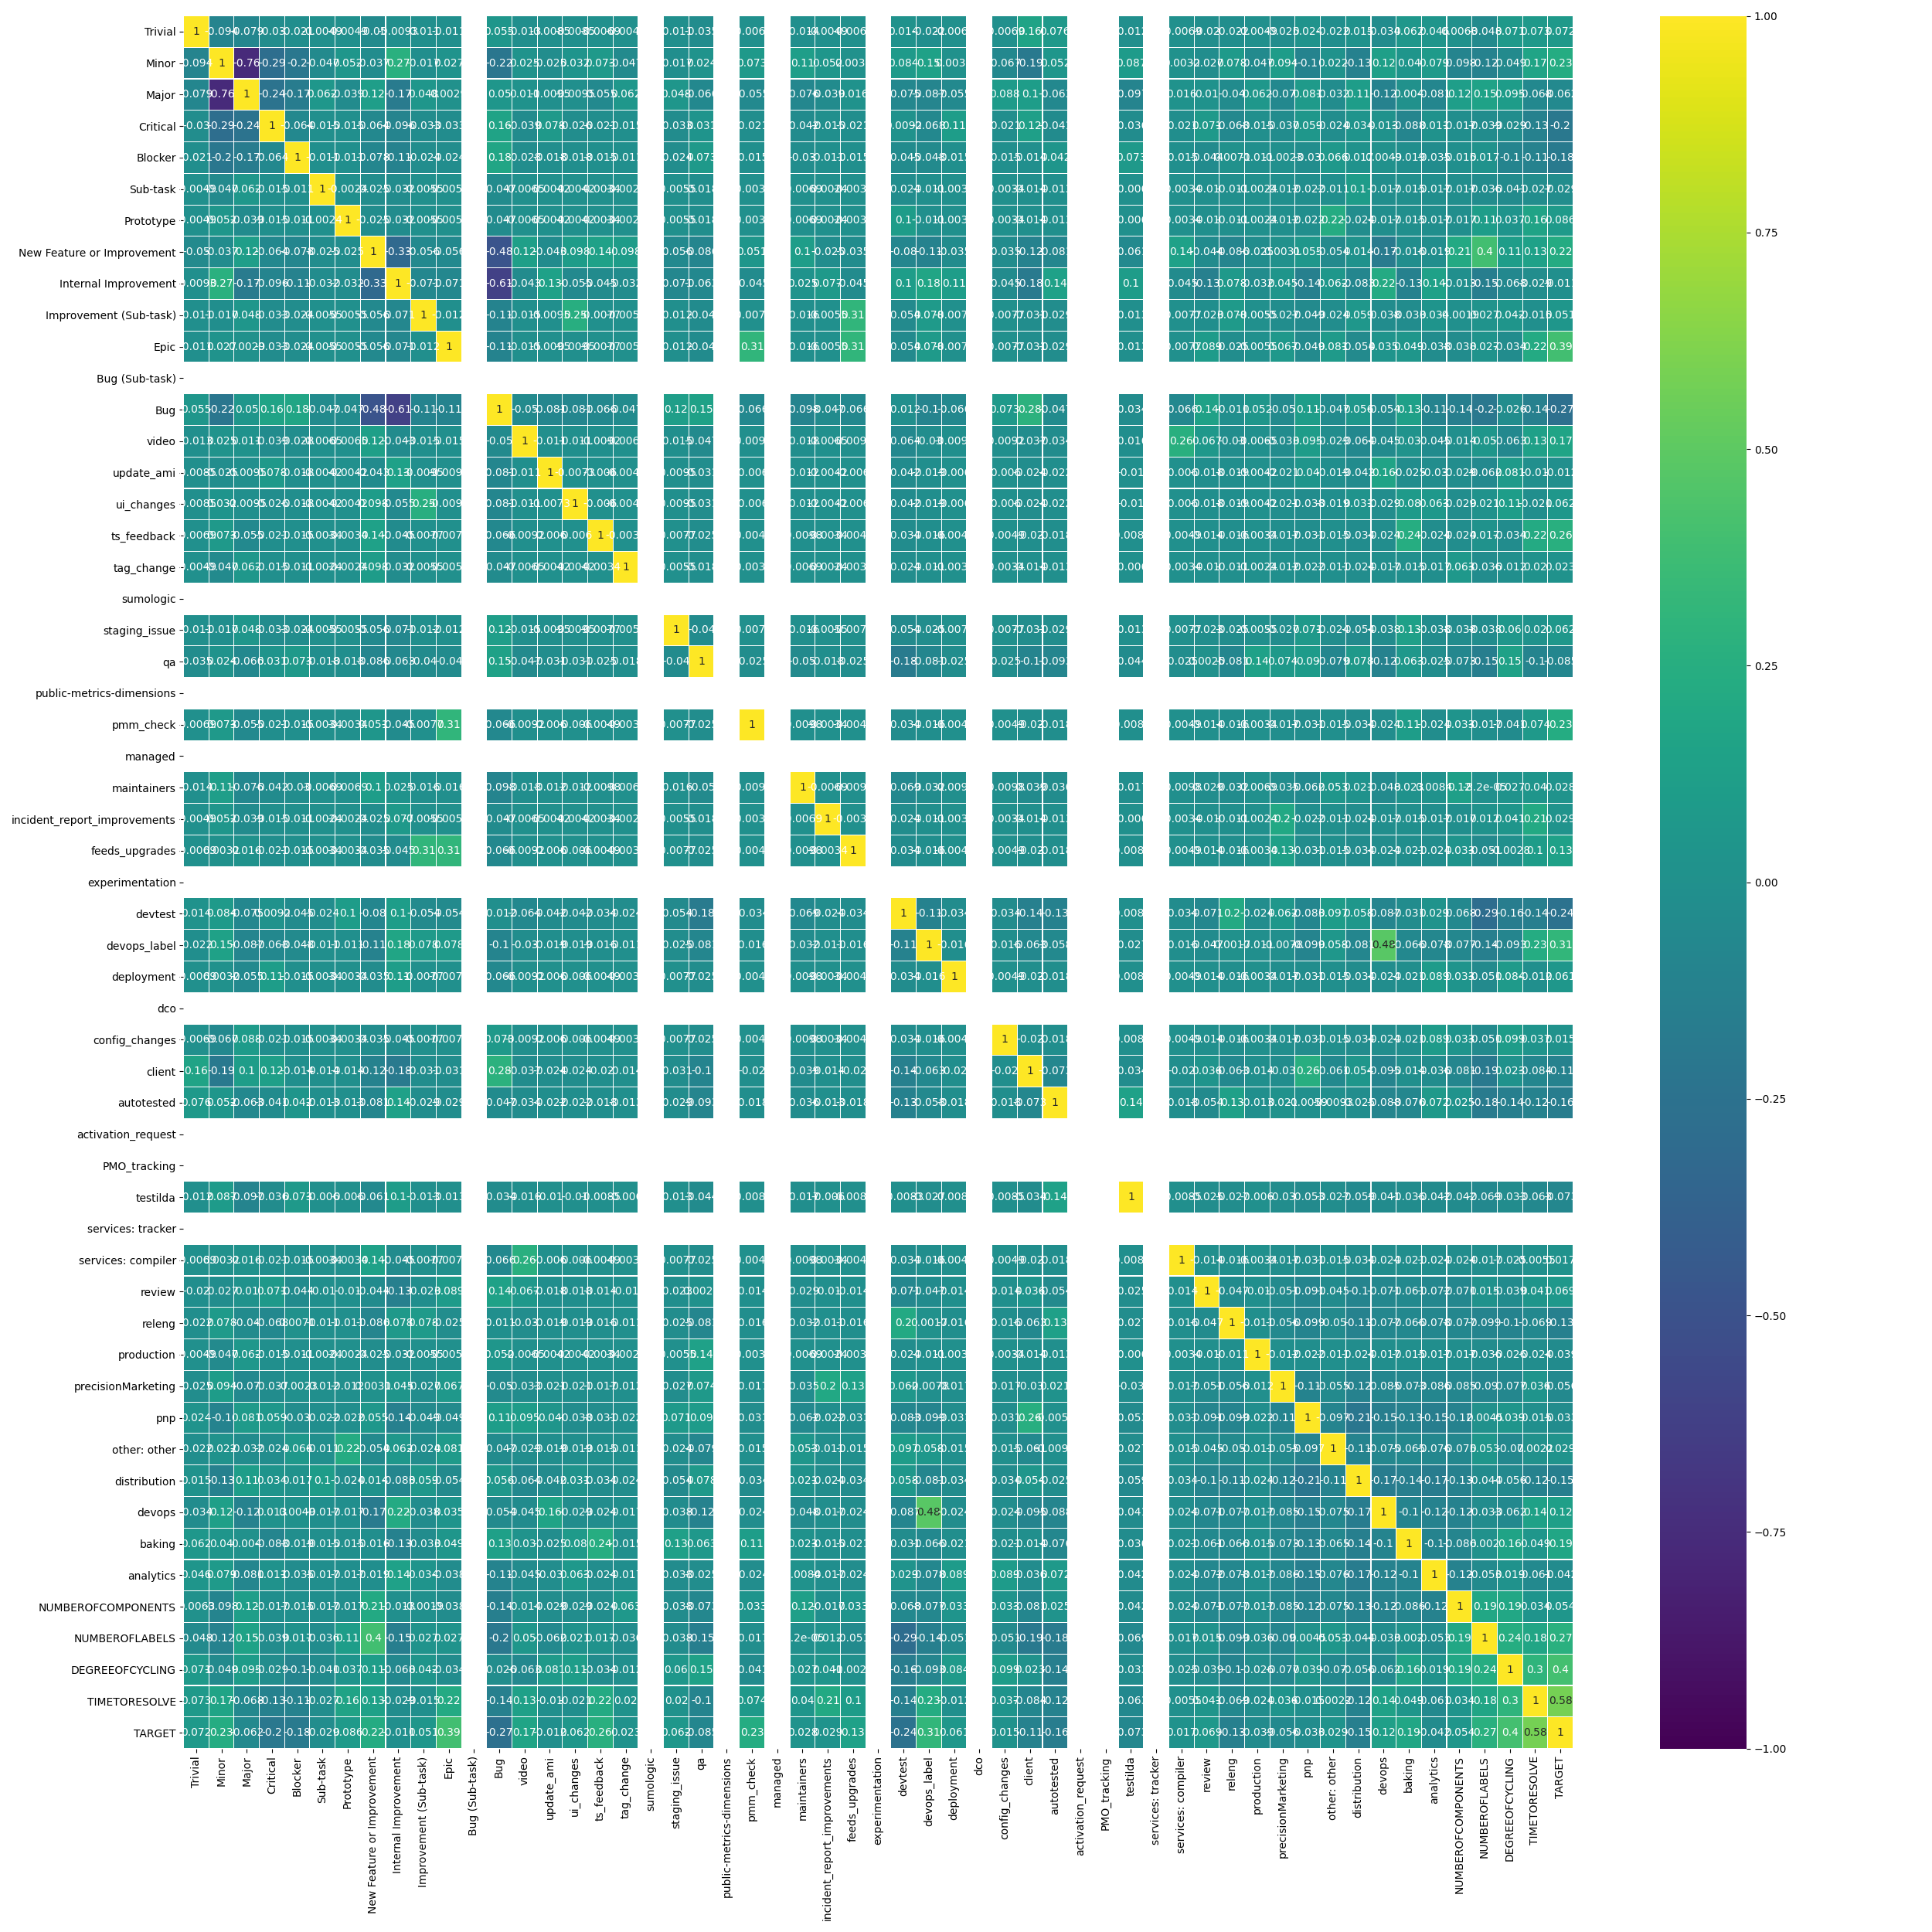
\includegraphics[width=2.5in]{feature_correlation.png}
\caption{Simulation results for the network.}
\label{fig_sim}
\end{figure}

\begin{figure*}[!t]
\centering
\subfloat[Case I]{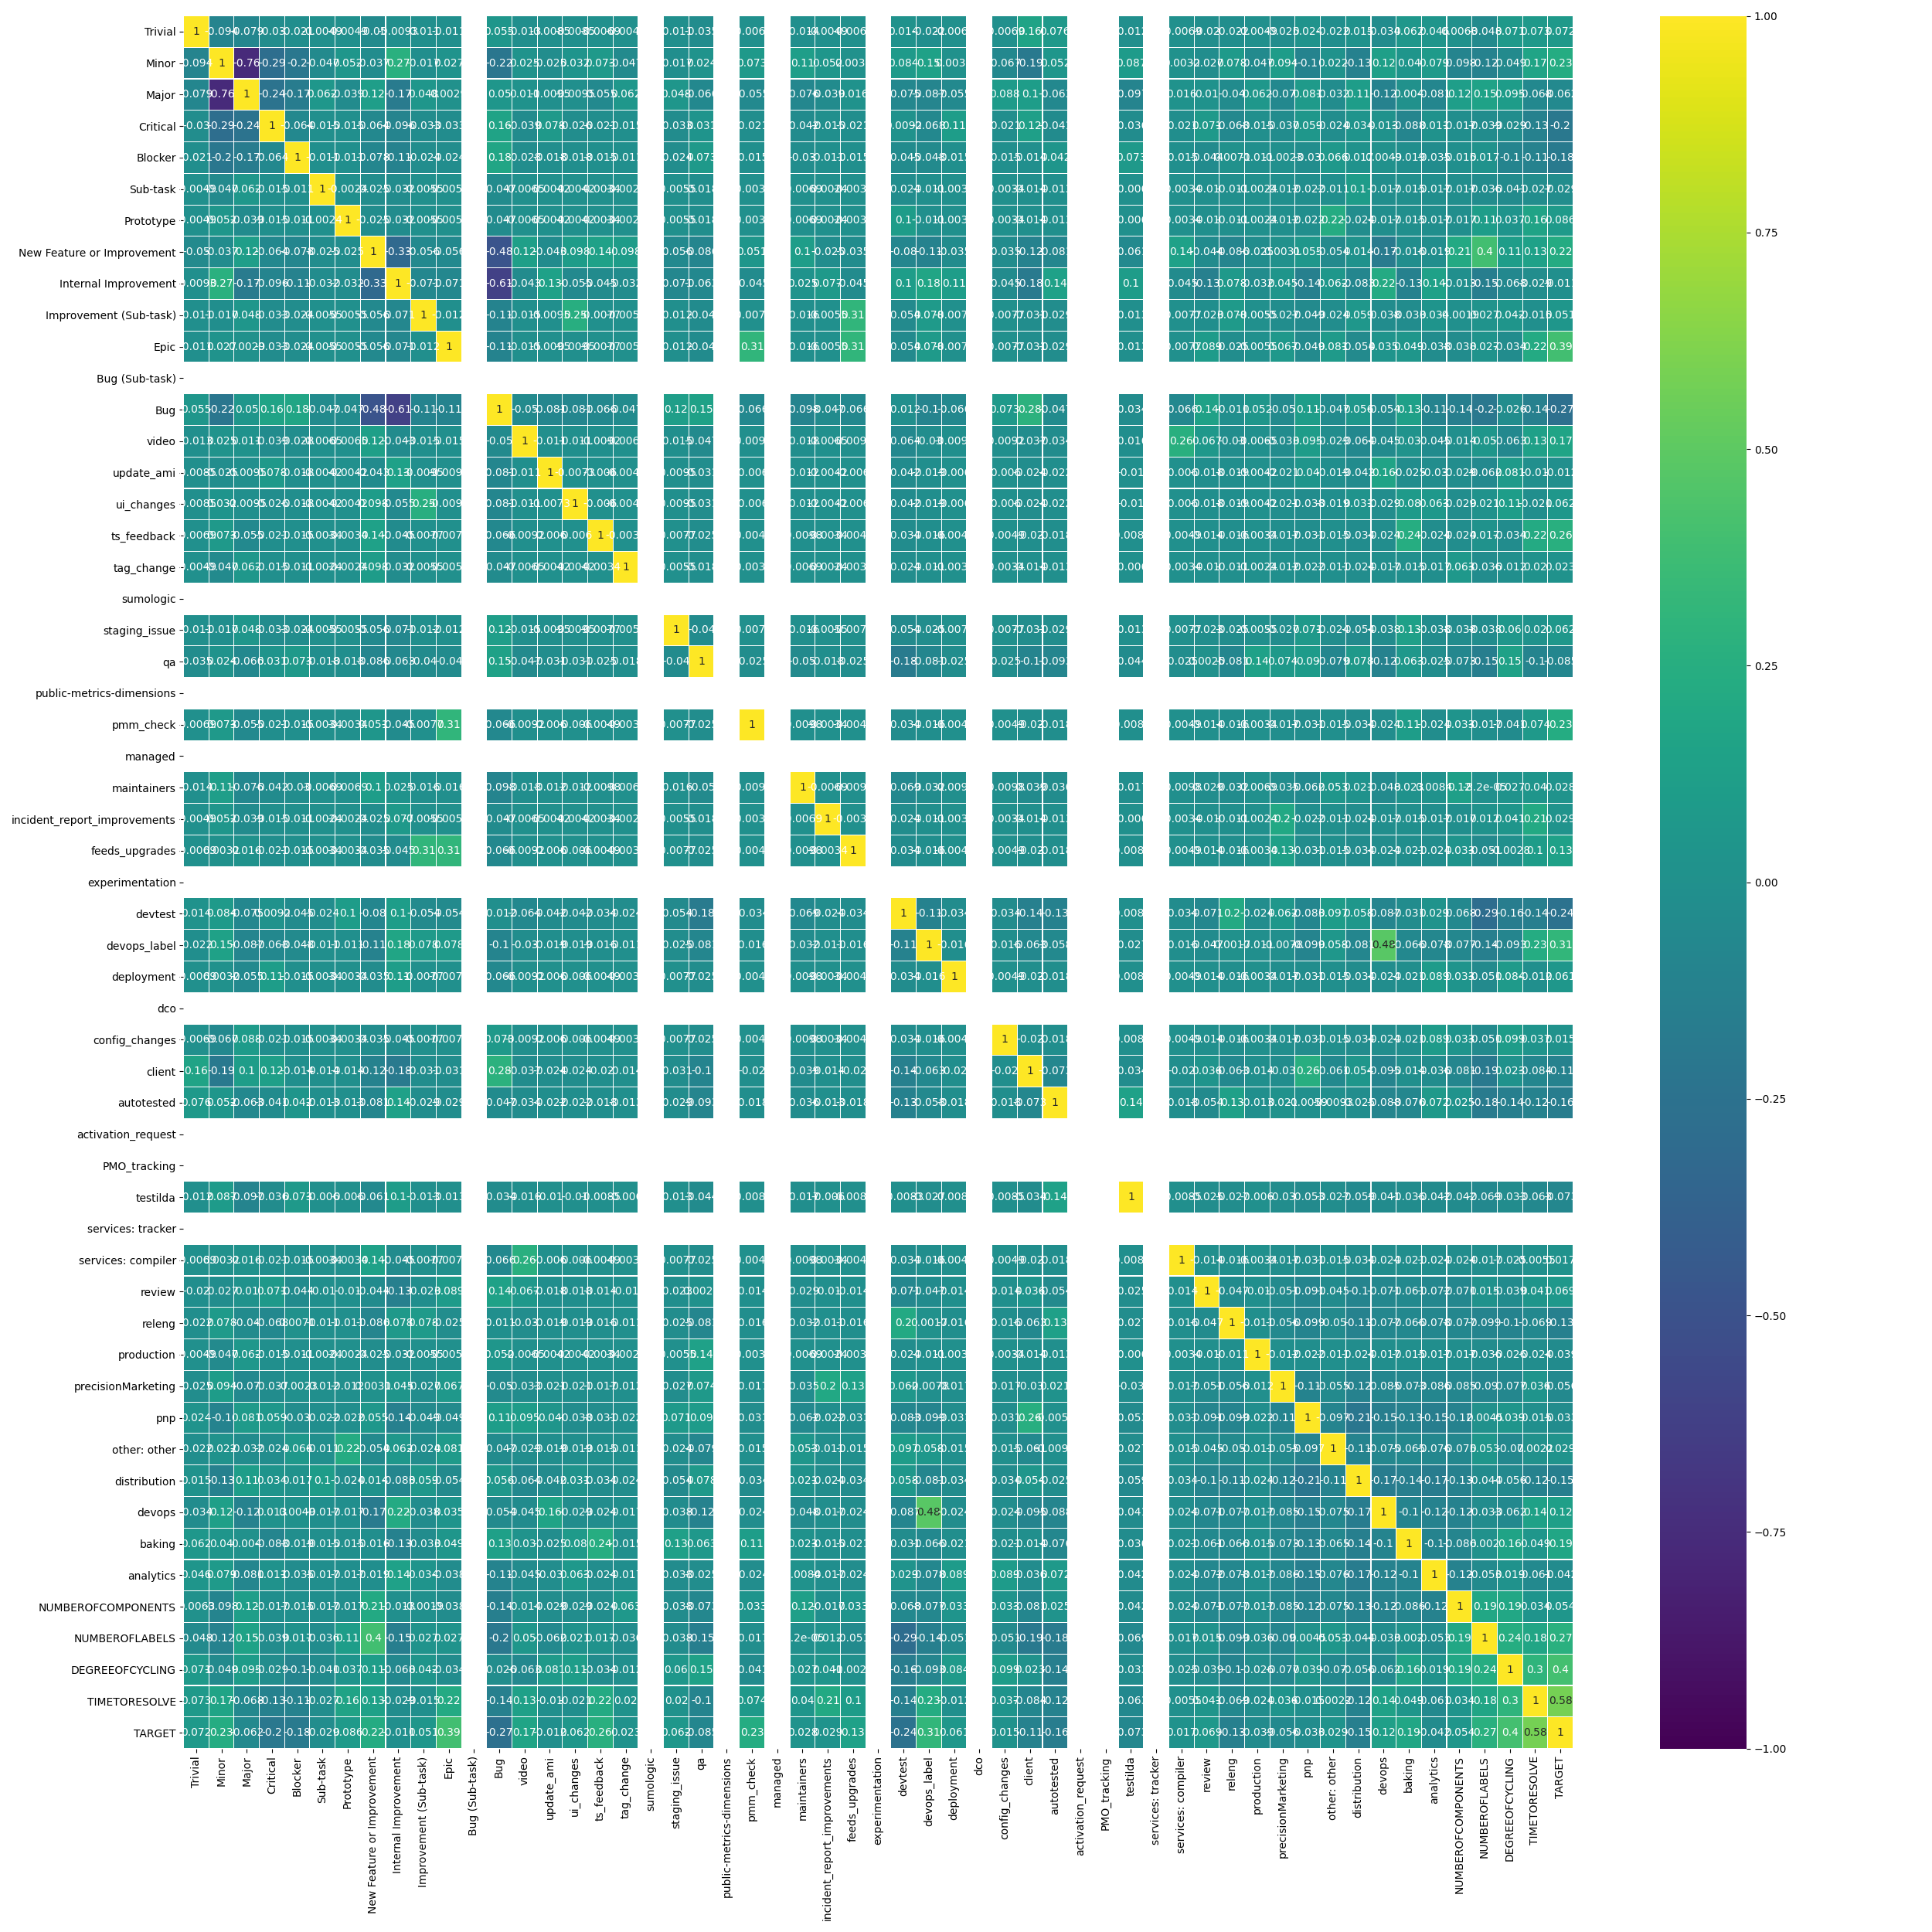
\includegraphics[width=2.5in]{feature_correlation.png}%
\label{fig_first_case}}
\hfil
\subfloat[Case II]{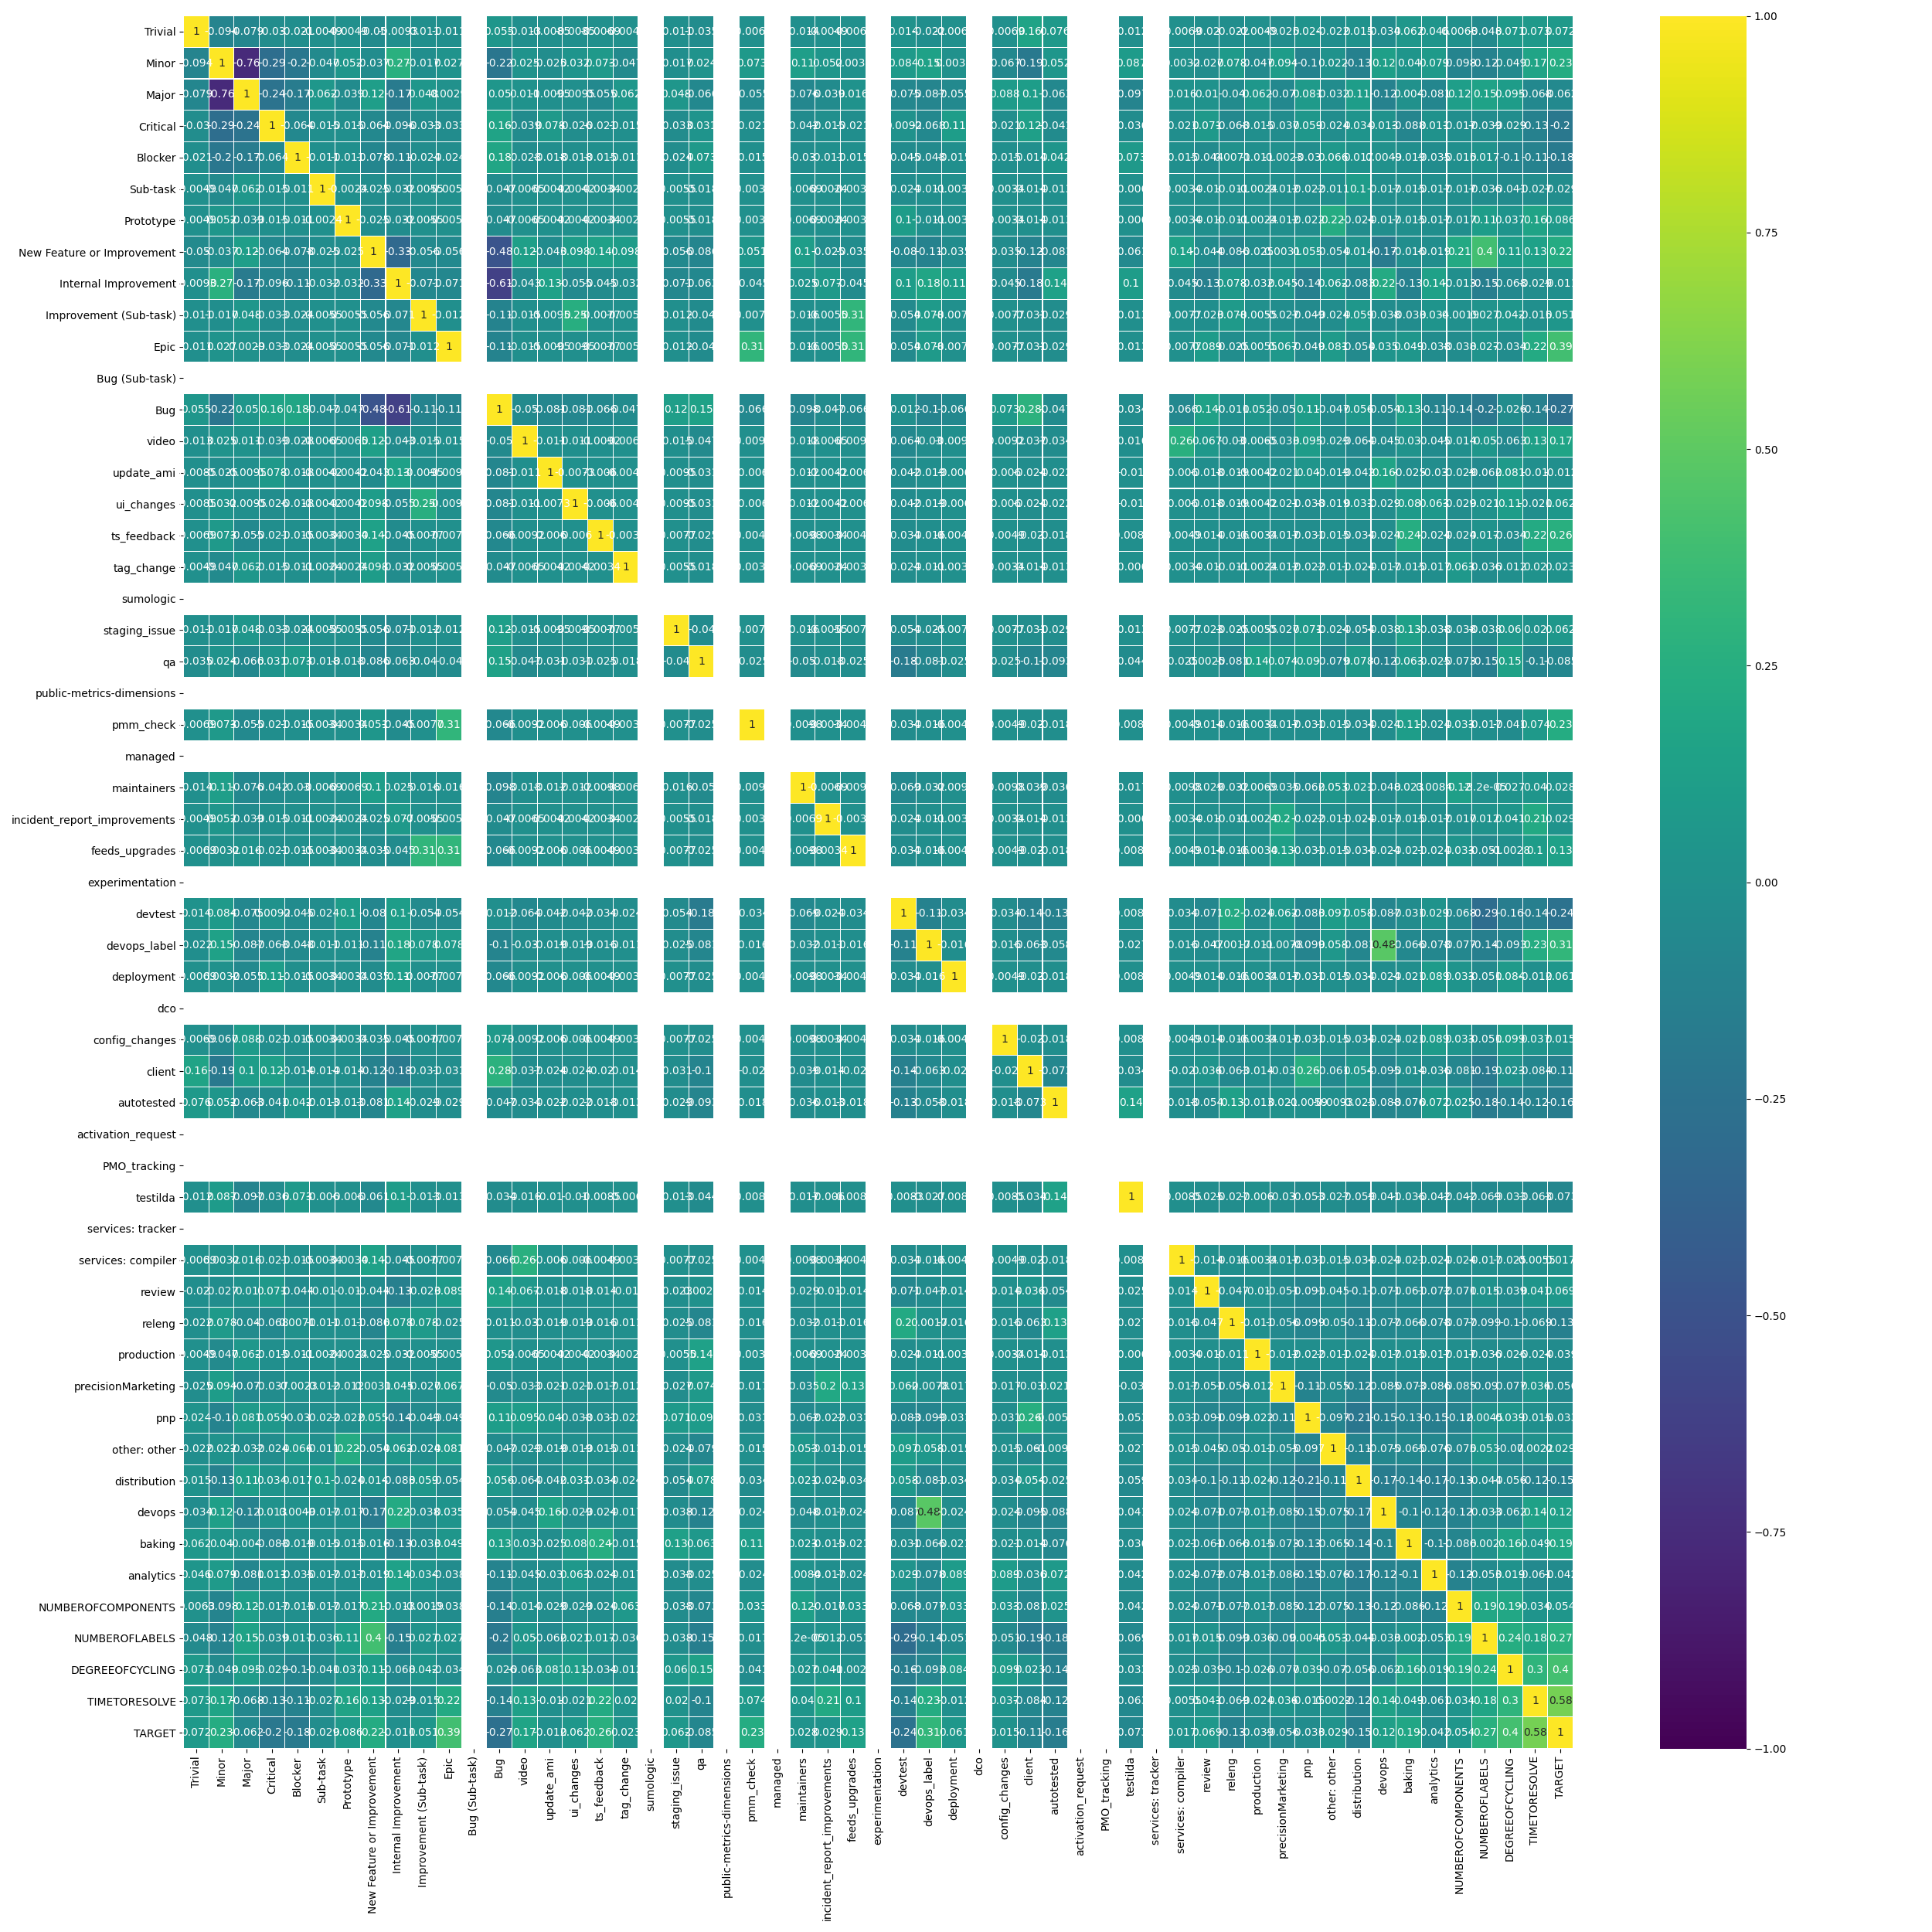
\includegraphics[width=2.5in]{feature_correlation.png}%
\label{fig_second_case}}
\caption{Simulation results for the network.}
\label{fig_sim2}
\end{figure*}

\begin{table}[!t]
\renewcommand{\arraystretch}{1.3}
\caption{An Example of a Table}
\label{table_example}
\centering
\begin{tabular}{|c||c|}
\hline
One & Two\\
\hline
Three & Four\\
\hline
\end{tabular}
\end{table}

\bibliographystyle{IEEEtran}
\bibliography{./references}
\end{document}


